\chapter{Germanium Compounds and QM Concerns}
\label{ch:Germanium}

\section{Modeling Germanium Compounds}

While primarily used in optical applications including fiber optic cables and solar cell systems, germanium-based compounds are also used as polymerization catalysts.
Relative to many other elements on the periodic table, computational reports on germanium are not common.
Recent works have shown germanium's potential to polarize light.

% This will be an interesting section as there is extremely little in terms of Ge computational work. Perhaps a broader search will yield interesting results. For sake of thoroughness, I will also include work on computational energy optimization in general and work through complications brought by the size of Ge. I might also include a portion on the statistical spread of conformations at a given temperature (internal energy?) I may include a sentence or paragraph on Gaussian-based publications. 

\subsection{Computational Complexity of Germanium Compounds}

Publications on germanium computational efforts are not as common as many other main group elements. 
Of those extant publications, the majority of final published data involve a Density Functional Theory (DFT) with either the 6-31G(d), 6-31G(d,p), or 6-311G(2d) basis set.\cite{GeCompStudy1}
As with most other lighter elements calculated with Pople basis sets, the 6-31G(d,p) basis set is most commonly used for the final energy calculation.
% WHY THIS? 
% D AND P POLARIZATION INCLUDED IN CALCULATION - WHAT DOES THIS MEAN?

\section{The Initial Problem: Germanium Study}

During Fall 2017, Dr. Christopher Fennell was approached by Dr. Charles Weinert of OSU to continue a collaborative effort in sampling conformation energies of two germanium-based compounds of interest to Dr. Weinert's work. 
Seen as an opportunity to train a new graduate student in conformational calculations, this project was delegated to me.
The initial focus was to create the two compounds in a 3D modeling program, save a file of each, run a conformation optimization program on a supercomputer, and read the output to report the findings.
As detailed below, this work led to impossibilities, curiosities, and inconsistencies that resulted in a general solution and a discovery of a flaw in a popular computational program.

\subsection{Parameters of Work and Previous Collaborator's Results}

The two subject germanium-based compounds are very similar: a germanium backbone with terminal isopropyl groups and internal phenyl rings. 
One compound constituted a pentagermanium chain while the other a hexagermanium backbone. 
The molecular formula for both is $Pr^{i}_{3}Ge(GePh_{2})_{n}GePr^{i}_{3}$ where n equals 3 for the pentagermanium or 4 for the hexagermanium compounds, respectively.
An example image of both compounds in their fully-trans configurations are provided in figures \ref{fig:Ge5TransAll} and \ref{fig:Ge6TransAll}.

\begin{figure}
	
	\centering
	
	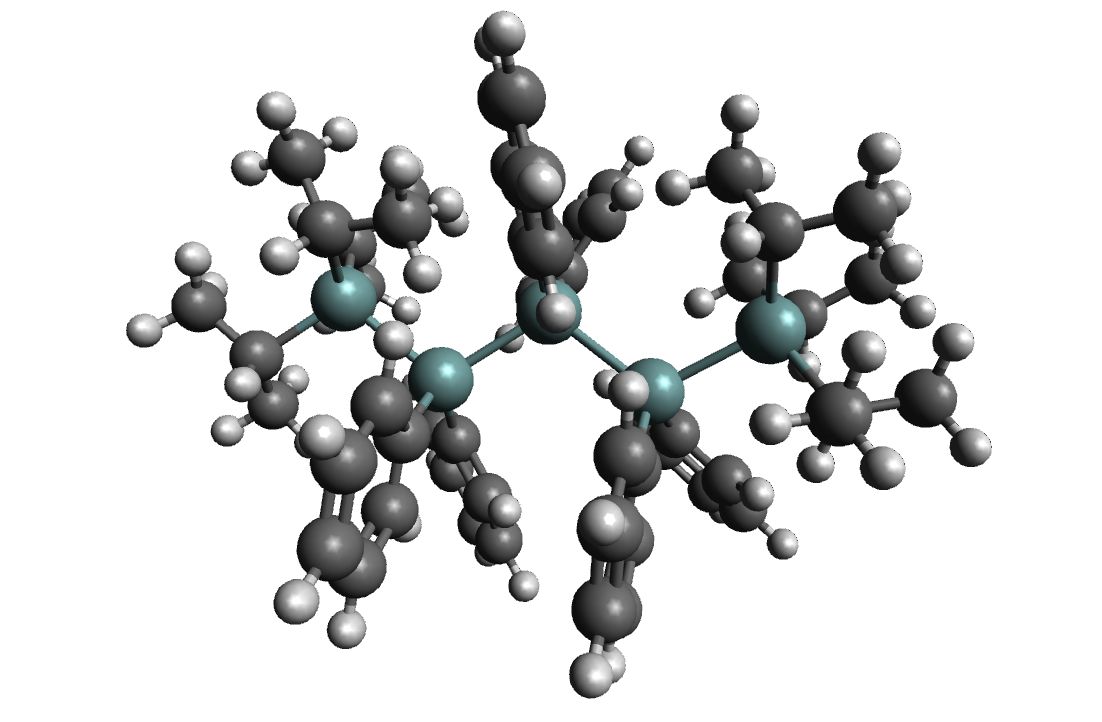
\includegraphics[width=0.75\textwidth]{5geTTT.png}
	
	\caption{Fully trans configuration of pentagermanium-based compound.}
	
	\label{fig:Ge5TransAll}
	
\end{figure}

\begin{figure}
	
	\centering
	
	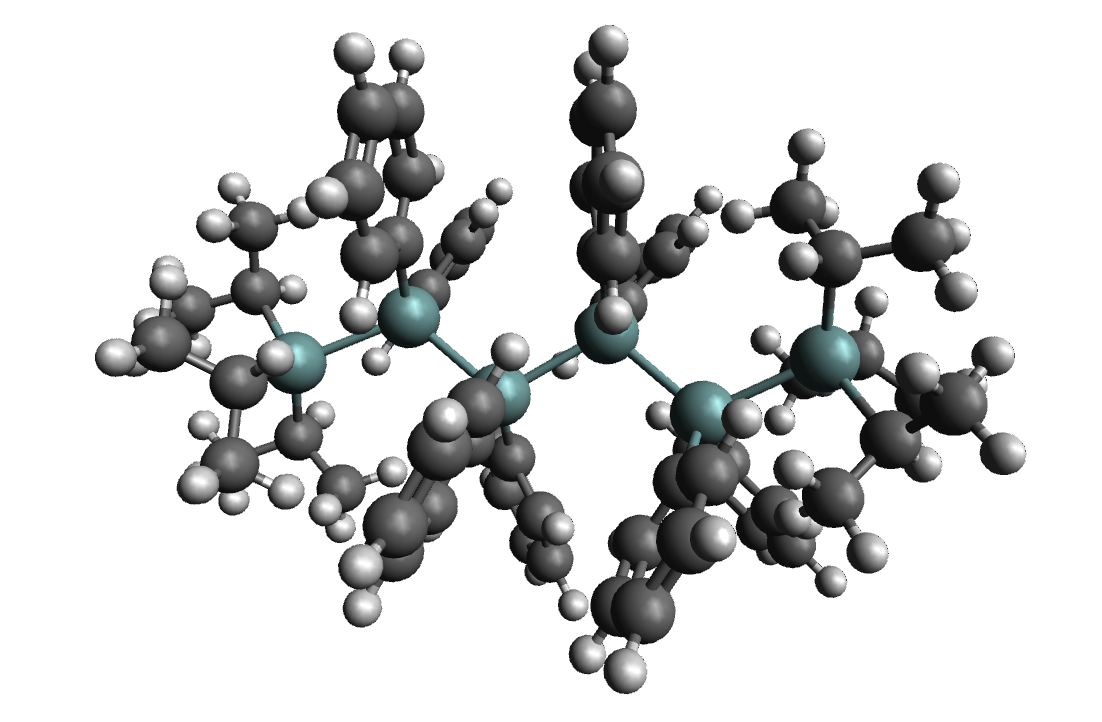
\includegraphics[width=0.75\textwidth]{6geTTT.png}
	
	\caption{Fully trans configuration of hexagermanium-based compound.}
	
	\label{fig:Ge6TransAll}
	
\end{figure}
\begin{table}[]
	
	\centering
	\begin{tabular}{llll}
		Conformation & Energy ($E_{h}$)    & $\Delta$ Energy ($E_{h}$) & $\Delta$ Energy ($\frac{kJ}{mol}$) \\ \cline{1-4} 
		Trans-coplanar        & -15014.8403143 & 0.0066255            & 17.39525025                        \\
		Cis-Trans-Cis         & -15014.7983311 & 0.0486087            & 127.6221418                        \\
		Trans-Cis-Trans       & -15014.8469398 & 0.0000000            & 0.0000000                                  \\
		Cis-Trans-Trans       & -15014.8246918 & 0.0222480            & 58.412124                         
	\end{tabular}
	\caption{Collaborator's Hexagermanium Energies by Conformation \\ (density functional theory, unknown basis set, energy in Hartrees and kJ/mol)}
	
	\label{tab:Ge6CollabEnergies}
	
\end{table}
Dr. Weinert had worked previously with a collaborator who provided conformation data supplied in table \ref{tab:Ge6CollabEnergies}.
While the basis set was not explicitly provided, it is likely that the most common 6-31G(d,p) basis set was used. 
Unfortunately, the collaborator is no longer active in research and was inaccessible for clarification.

The approach of labeling the conformation shape of each compound, given the many points of torsion, focuses on the backbone structure. 
As the raw data from the collaborator was not available, the general dihedral angles of cis and trans proved a vexing focus for initial efforts at conformer design.
Using Newman projections like in figure \ref{fig:Newman} as a visual guide, each Ge-Ge bond was defined as cis or trans based on the relative angle produced by the two  adjacent bonded Ge atoms to each subject Ge.
Specifically, the bonds are marked cis if the most acute angle is 90$^{\circ}$ or fewer, and likewise trans if greater than 90$^{\circ}$ up to the maximum 180$^{\circ}$.
Effectively the cis and trans angles coincide with gauche and anti in organic structure nomenclature.
Terminal germanium atoms are not considered as a part of the conformation state. 
This is partly due to the definition in labeling where the terminal germanium does not have an adjacent germanium for the measured relative angle, in addition to the assumed 
% CONFIRM GROUP THEORY - possibly S3?
C$_{3}$
% CONFIRM GROUP THEORY
symmetry of the terminal Ge with three isopropyl groups reducing the relative effects of terminal germanium rotation.
Effectively, only dihedrals formed by four consecutive Ge are given a cis or trans label.

\begin{figure}
	
	\centering
	
	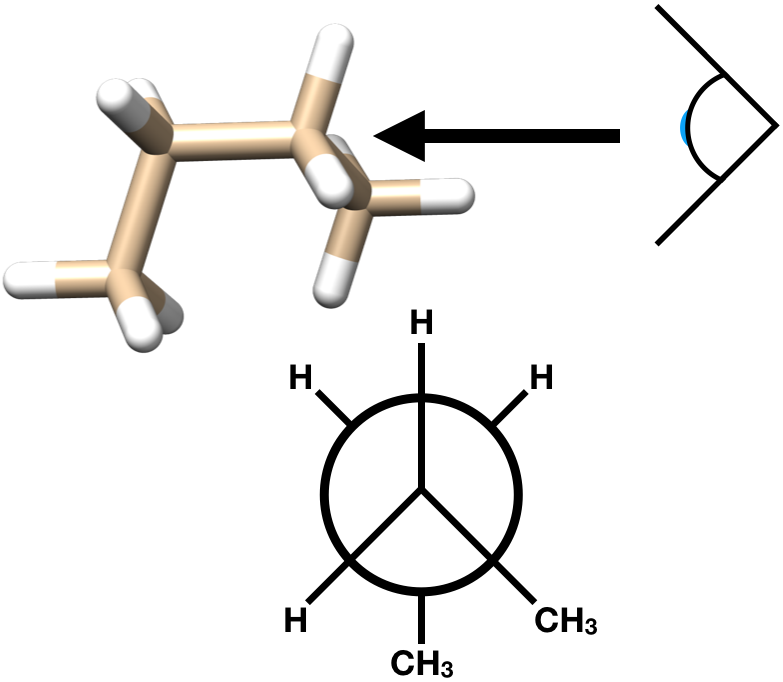
\includegraphics[width=0.75\textwidth]{NewmanCis.png}
	
	\caption{Sample Newman projection of cis-butane.}
	
	\label{fig:Newman}
	
\end{figure}

\subsection{Design and Approach to Solution}

The initial approach involved an attempt at basic replication of the collaborative results.
As detailed below, the design gradually grew in complexity as a learning process. 
Eventually, curiosities in results and a desire to automate an objective search algorithm developed into two unique investigations.

\subsubsection{Design 1: Occam's Smallest Razor}

With each non-terminal Ge-Ge dihedral initially labeled cis or trans for 0$^{\circ}$ or 180$^{\circ}$, about 3 unique pentagermanium and 6 unique hexagermanium structures were built visually on a 3D visualization program (Avogadro).
These were rotated without consideration for the phenyl rings populating the non-terminal Ge atoms.
Each molecule was subjected to an energy minimization in Gaussian 09 with the B3LYP hybrid function and STO-3G basis set as a single particle in a vacuum at otherwise default settings. 

Unsurprisingly, only the fully trans conformers successfully converged (a 22\% success rate) into a stable form. 
These troubles were likely caused by the poor design of the initial conformers. 
With initial results, the conformer design was altered into a more systematic approach with some consideration for the phenyl rings.

\subsubsection{Design 2: A Blunt Effort}

In the second iteration of the conformer design process, a greater number of backbone conformers were generated. 
Instead of the simple 180$^{\circ}$ opposition between the cis and trans conformers, more intentional initial angles seen in Newman projections were selected.
Specifically, the anti and both gauche angles were chosen for the natural local minima in a non-bulky molecule, with both gauche angles (60 and 300) labeled as cis and the anti angle (180) as trans. 
For initial conformer design, these backbone angles were limited to three positions: 60$^{\circ}$, 180$^{\circ}$, or 300$^{\circ}$.
For the hexagermanium compound, these structures were sequentially labeled trans-trans-trans, trans-trans-cis, trans-cis-trans, et cetera until all major unique conformers were produced.
For clarity, each conformer was identified by the dihedral angles (60-60-60, 60-60-180) in increasing order (Ge 1-2-3-4, Ge 2-3-4-5, Ge 3-4-5-6 dihedral).
The phenyl rings on the non-terminal Ge atoms were left untouched from an initial steepest-descent minimization available from Avogadro ran in the fully trans conformer.

To prevent potentially strong interactions between adjacent phenyl rings, an additional steepest-descent minimization from Avogadro was initially ran with the conformer-defining Ge-Ge dihedral angles locked in place. 
Additionally, a visual inspection of the phenyl rings and manual adjustments were utilized on Avogadro to reduce the chance of a relatively high energy local minima conformer. 
The phenyl rings usually were settled in a form of pi stacking or some kind of perpendicular ring interaction, based on relative energy stability according to the immediate simple minimization available. 

To further avoid backbone rotation restrictions, variations of the bulky molecules were also produced. 
These included versions where the phenyl rings were replaced by methyl groups and also where the isopropyl ends were additionally replaced by methyl groups. 
There intention in these designs were to observe the shift in relative energy between the sets of conformers to determine how significant of a role the phenyl rings and isopropyl groups played.
These variations, along with the original form structures, were subject to the same calculations as in the first design: Gaussian 09, B3LYP hybrid functional, STO-3G basis set, no angle restrictions, single particle in a vacuum, otherwise default parameters.
The results of these calculations are tabulated in tables \ref{tab:Ge5Ver2Data} and \ref{tab:Ge6Ver2Data}.

\begin{table}[]
	\centering
	\begin{tabular}{llllll}
		\begin{tabular}[c]{@{}l@{}}Internal\\ Species\end{tabular} & \begin{tabular}[c]{@{}l@{}}Terminal\\ Species\end{tabular} & Conformer & \begin{tabular}[c]{@{}l@{}}Final Energy\\ (Hartrees)\end{tabular} & \begin{tabular}[c]{@{}l@{}}∂ Energy\\ (Hartrees)\end{tabular} & \begin{tabular}[c]{@{}l@{}}∂ Energy\\ (kJ/mol)\end{tabular} \\ \hline
		methyl & methyl & 60-60 & -10738.91336 & 0.0000454 & 0.119 \\
		methyl & methyl & 60-180 & -10738.9134 & 0 & 0 \\
		methyl & methyl & 60-300 & -10738.91286 & 0.0005358 & 1.407 \\
		methyl & methyl & 180-60 & -10738.91325 & 0.0001533 & 0.402 \\
		methyl & methyl & 180-180 & -10738.91335 & 0.0000475 & 0.125 \\
		methyl & methyl & 180-300 & -10738.91336 & 0.0000451 & 0.118 \\
		methyl & methyl & 300-60 & -10738.91336 & 0.0000455 & 0.119 \\
		methyl & methyl & 300-180 & -10738.91287 & 0.0005357 & 1.406 \\
		methyl & methyl & 300-300 & -10738.9107 & 0.002703 & 7.097 \\ \hline
		phenyl & methyl & 60-60 & -11875.15183 & 0.0001451 & 0.381 \\
		phenyl & methyl & 60-180 & -11875.15144 & 0.0005304 & 1.393 \\
		phenyl & methyl & 60-300 & -11875.15197 & 0 & 0 \\
		phenyl & methyl & 180-60 & -11875.14282 & 0.0091505 & 24.025 \\
		phenyl & methyl & 180-180 & -11875.15004 & 0.0019354 & 5.081 \\
		phenyl & methyl & 180-300 & -11875.15064 & 0.0013353 & 3.506 \\
		phenyl & methyl & 300-60 & -11875.06665 & 0.0853257 & 224.023 \\
		phenyl & methyl & 300-180 & DNC & DNC & DNC \\
		phenyl & methyl & 300-300 & -11875.1497 & 0.0022723 & 5.966 \\ \hline
		phenyl & isopropyl & 60-60 & DNC & DNC & DNC \\
		phenyl & isopropyl & 60-180 & -12341.23176 & 0.0053028 & 13.923 \\
		phenyl & isopropyl & 60-300 & DNC & DNC & DNC \\
		phenyl & isopropyl & 180-60 & DNC & DNC & DNC \\
		phenyl & isopropyl & 180-180 & -12341.23513 & 0.001935 & 5.08 \\
		phenyl & isopropyl & 180-300 & DNC & DNC & DNC \\
		phenyl & isopropyl & 300-60 & DNC & DNC & DNC \\
		phenyl & isopropyl & 300-180 & -12341.23706 & 0 & 0 \\
		phenyl & isopropyl & 300-300 & DNC & DNC & DNC
	\end{tabular}
	\caption{Data of B3LYP/STO-3G minimization of variations of pentagermane compound at various conformers. DNC denotes a failure to converge with the self-consistent field method.}
	\label{tab:Ge5Ver2Data}
\end{table}

\begin{table}[]
	\centering
	\begin{tabular}{llllll}
		\begin{tabular}[c]{@{}l@{}}Internal\\ Species\end{tabular} & \begin{tabular}[c]{@{}l@{}}Terminal\\ Species\end{tabular} & Conformer & \begin{tabular}[c]{@{}l@{}}Final Energy\\ (Hartrees)\end{tabular} & \begin{tabular}[c]{@{}l@{}}∂ Energy\\ (Hartrees)\end{tabular} & \begin{tabular}[c]{@{}l@{}}∂ Energy\\ (kJ/mol)\end{tabular} \\ \hline
		methyl & methyl & 60-60-60 & -12870.91834 & 0.0009503 & 2.495 \\
		methyl & methyl & 60-180-60 & -12870.91929 & 0.0000004 & 0.001 \\
		methyl & methyl & 60-180-180 & -12870.91813 & 0.0011628 & 3.053 \\
		methyl & methyl & 60-180-300 & -12870.91869 & 0.0005972 & 1.568 \\
		methyl & methyl & 60-300-300 & DNC & DNC & DNC \\
		methyl & methyl & 180-60-60 & -12870.91897 & 0.0003189 & 0.837 \\
		methyl & methyl & 180-180-60 & -12870.91833 & 0.0009585 & 2.517 \\
		methyl & methyl & 180-180-180 & -12870.91929 & 0.0000004 & 0.001 \\
		methyl & methyl & 180-180-300 & -12870.91929 & 0.0000003 & 0.001 \\
		methyl & methyl & 180-300-60 & -12870.91897 & 0.0003192 & 0.838 \\
		methyl & methyl & 300-60-180 & DNC & DNC & DNC \\
		methyl & methyl & 300-180-60 & -12870.91929 & 0 & 0 \\
		methyl & methyl & 300-180-180 & DNC & DNC & DNC \\
		methyl & methyl & 300-180-300 & -12870.91814 & 0.0011527 & 3.026 \\ \hline
		phenyl & methyl & 60-60-60 & DNC & DNC & DNC \\
		phenyl & methyl & 60-60-180 & -14385.89674 & 0.0052183 & 13.701 \\
		phenyl & methyl & 60-60-300 & -14385.89487 & 0.0070829 & 18.596 \\
		phenyl & methyl & 60-180-60 & DNC & DNC & DNC \\
		phenyl & methyl & 180-60-60 & DNC & DNC & DNC \\
		phenyl & methyl & 180-60-180 & -14385.90195 & 0 & 0 \\
		phenyl & methyl & 180-60-300 & -14385.89855 & 0.0033998 & 8.926 \\
		phenyl & methyl & 180-180-180 & -14385.83838 & 0.0635763 & 166.92 \\
		phenyl & methyl & 180-300-180 & -14385.79233 & 0.1096251 & 287.821 \\
		phenyl & methyl & 300-60-60 & DNC & DNC & DNC \\
		phenyl & methyl & 300-60-180 & -14385.89836 & 0.003597 & 9.444 \\
		phenyl & methyl & 300-60-300 & -14385.89836 & 0.0035979 & 9.446 \\
		phenyl & methyl & 300-180-60 & DNC & DNC & DNC \\
		phenyl & methyl & 300-300-300 & DNC & DNC & DNC \\ \hline
		phenyl & isopropyl & 60-180-180 & -14851.9865 & 0 & 0 \\
		phenyl & isopropyl & 60-300-60 & DNC & DNC & DNC \\
		phenyl & isopropyl & 60-300-180 & DNC & DNC & DNC \\
		phenyl & isopropyl & 180-300-60 & DNC & DNC & DNC \\
		phenyl & isopropyl & 180-300-180 & DNC & DNC & DNC \\
		phenyl & isopropyl & 180-300-300 & DNC & DNC & DNC \\
		phenyl & isopropyl & 300-300-60 & DNC & DNC & DNC \\
		phenyl & isopropyl & 300-300-180 & DNC & DNC & DNC \\
		phenyl & isopropyl & 300-300-300 & DNC & DNC & DNC
	\end{tabular}
	\caption{Data of B3LYP/STO-3G minimization of variations of hexagermane compound at various conformers. DNC denotes a failure to converge with the self-consistent field method.}
	\label{tab:Ge6Ver2Data}
\end{table}


Immediately obvious in the table are the considerable number of nonconverged results. 
An unexpected bulkiness trend followed that a fully methylated variation of the structure was most likely to converge to a stable state, while the fully internal phenyl structures with methyl ends slightly reduced convergence and the original fully internal phenyl structures with isopropyl ends drastically reduced convergence.
The common-sense expectation that the addition of the phenyl ends would reduce stability was not parroted in these results. 
A deeper exploration into the change of stability is a promising avenue for future investigation, but was not further explored in this work.
As can be seen in table \ref{tab:Ge6Ver2Data}, the lowest energy conformer for each structure varied greatly, but never included the fully trans conformer and only once the collaborator-reported trans-cis-trans conformer as the most stable.
Still, given the considerable amount of nonconverged conformers, a new design was necessary to further improve the scope of the lowest energy conformation search.

\subsubsection{Design 3: Death by 1.59 Million Cuts}

In the final version of the conformer generation effort, additional creation efforts were focused on the individual phenyl rings. 
The unfavorable interactions between the phenyl rings were considerable hurdle in the previous designs and a potential explanation for the large number of nonconverged structures, including the possibility that the terminal isopropyl hexagermanium structures contained particularly unfavorable interactions among the phenyl rings.
This third design sought to remove the uncertainty in phenyl ring bulkiness by applying the same approach as the backbone generation: create unique conformers of every backbone torsion and phenyl ring, limiting each torsion to one of three rotational positions following the Newman projection style. 
Unfortunately, this task proved prohibitively large.

As an explanation for the insurmountability of the problem, consider the hexagermanium structure. 
The germanium dihedrals represent three rotatable bonds each with three initial positions. 
To include the phenyl rings would require the inclusion of eight new rotatable bonds each with three initial positions.
Additionally, considering each terminal germanium's rotation while ignoring each isopropyl's rotatable bonds adds two initial positions each with three initial positions. 
Together, this creates a structure with 13 rotatable bonds each with three initial positions. The number of conformers follows as $3^{13} = 1,594,323$ initial conformers. 
Now we must consider the computational aspect of this many conformers.
At 10 conformers rotated and generated per second and 16 KB per conformer, the initial conformers would require 44.3 hours and generate 25.49 GB of data just in the initial structures.
At an average of 72 minutes per computation and 73.7 MB produced at B3LYP hybrid functional and STO-3G basis set and access to all 255 regular nodes of Oklahoma State University's Cowboy cluster running in parallel, the complete computation would generate 117.5 TB of data and require 312 days of continuous computation to determine a possible lowest energy conformer of this one molecule at a relatively low level basis set and theory.
A request to utilize 100\% of university supercomputer resources for nearly a year for the sake of determining the lowest energy conformer of one molecule would likely be rejected, so this task would likely require a time scale of years or even decades to produce with shared access to university resources. 
While conventionally considered a small molecule, the scale of conformers and computational requirements pushes this problem into the realm of Levinthal's paradox.

While this third design would have likely revealed the lowest energy conformer, or at least one considerably close the the exactly lowest energy conformer, the effort ultimate fails under its own weight.
Even with efforts to truncate duplicate forms, the problem of scale remains.
A reduction by 50\% still requires a computation effort in the timescale of years or decades for the calculation of a single molecule.
For an effective computational outlook, this system needs to be reduced by several orders of magnitude.

\subsection{Scale Reduction Efforts}

For a system with conformers on the millions scale and computations on the hour scale, a magnitude reduction in either aspect would improve the practicality of this design approach.
For example, by simplifying the computational method from 72 minutes on average to 5 minutes on average, the overall computational requirement would be reduced by 92\%, a full order of magnitude. 
Unfortunately, reducing the complexity of the method sacrifices the reliability of data.
A potential solution here would be to create rounds of calculations at different complexities, where each sequential round restricts the pool of potential conformers.
Ideally, the balance of the increasing computational complexity and the decreasing pool size would maintain a consistent computational requirement.
For example, a new round using a higher functional theory and basis set at 5x computational requirement would ideally be paired with a reduction in conformer pool size by a factor of 5.
This would produce a series of calculation sets with additive computational requirement instead of a magnitudinal expansion.

The natural next question lies within the reliability of basis sets and functional theories. 
It naturally follows that a less-accurate method should not be relied on while better methods exist. 
However, considering the scale of the conformer pool, it follows that a less accurate method would still produce energy values with a roughly similar internal consistency. 
For example, a 180-0-180 form of the hexagermanium compound with parallel phenyl rings as modeled in figure \ref{fig:6geTCT} will have intense syn interactions between some phenyl rings and will likely not yield a desirable energy value at any level of calculation while a fully trans form with perfect pi stacking phenyl rings will likely have a lower energy value at all levels of calculation.
It follows that, at lower levels of accuracy, the extremely high energy conformers can be pruned from the pool early and drastically reduce overall computational requirements.
A generic effort at producing a method in this style is detailed in chapter \ref{ch:ConformationLandscape}, while the remainder of this chapter details additional efforts of calculating these germanium compounds.

\begin{figure}
	
	\centering
	
	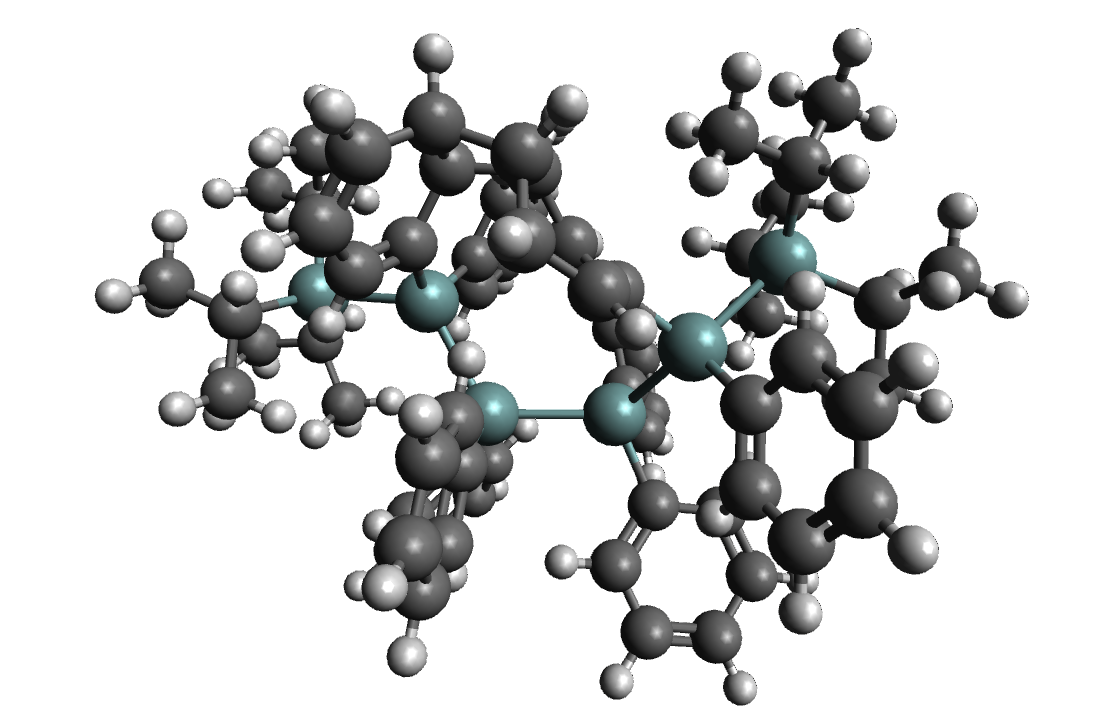
\includegraphics[width=0.75\textwidth]{6geTCT.png}
	
	\caption{Visualization of a trans-cis-trans hexagermane structure.}
	
	\label{fig:6geTCT}
	
\end{figure}

\subsection{Efforts at Simplification}

One potential avenue of simplifying the process is computing the energy minimizations of lower-period atoms (e.g. a carbon backbone instead of germanium) and then applying a correction factor for a net reduction in computation time.
As a period 4 element, germanium exhibits computational qualities similar to but more complicated than both carbon and silicon.
Using tested samples, an energy minimization of a carbon-backbone molecule instead of the germanium represented a 92\% reduction in computation speed.
Assuming a nominal correction factor exists and can be applied, this represents an order of magnitude reduction in computation time with one simplification. 
Potentially, this would allow investigators to much more quickly eliminate high energy conformers and more rapidly reduce the scope of the search.

The approach to acquiring sufficient data for a possible correction factor involved running an extremely simplified form of the germanium compounds, specifically a butagermanium backbone with hydrogens occupying all terminal and internal bonds.
This reduced the complication and complexity of bulkiness and allowed for quick full torsion rotations about the single Ge-Ge-Ge-Ge dihedral.
By operating at intervals of 5$^{\circ}$, a full torsion drive provides a glimpse at relative energies of the molecule at 72 discrete states. 

The extended round of torsion drive calculations included an alteration in representation of the data.
As the focus had shifted from relative energies and intensities across multiple theories and basis sets to a focus on graph smoothness and internal relative energies, the energy axis of plots were reduced to a unitless scale ranging 0 to 1, where 0 represents the minimum energy and 1 represents the maximum energy in a given set of torsion drive data.
This allowed for graphical representations of each torsion drive to emphasize the internal variation of torsions relative to the minimum and maximum values.
This was accomplished by taking any set of data with absolute scale energy unit, identifying the minimum and maximum values, and scaling each data point according to equation \ref{eq:TorsionReducedScale}. 
The script to collect and scale data points is detailed in \ref{ch:App:Germane}.

\begin{equation}
% NEEDS SOME WORK
E_{i, red} = \frac{E_{i,abs} - E_{min,abs}}{E_{max,abs}-E_{min,abs}}
\label{eq:TorsionReducedScale}
% NEEDS SOME WORK
\end{equation}

An example plot of this torsion drive is shown in figure \ref{fig:EXTorsion} Once multiple torsion drives had completed in multiple group four elements (butyl C, Si, and Ge were all built and tested), the energies could be compared and analyzed for any relative or absolute scaling at the additive or multiplicative reference. 
%MORE

\begin{figure}
	
	\centering
	
	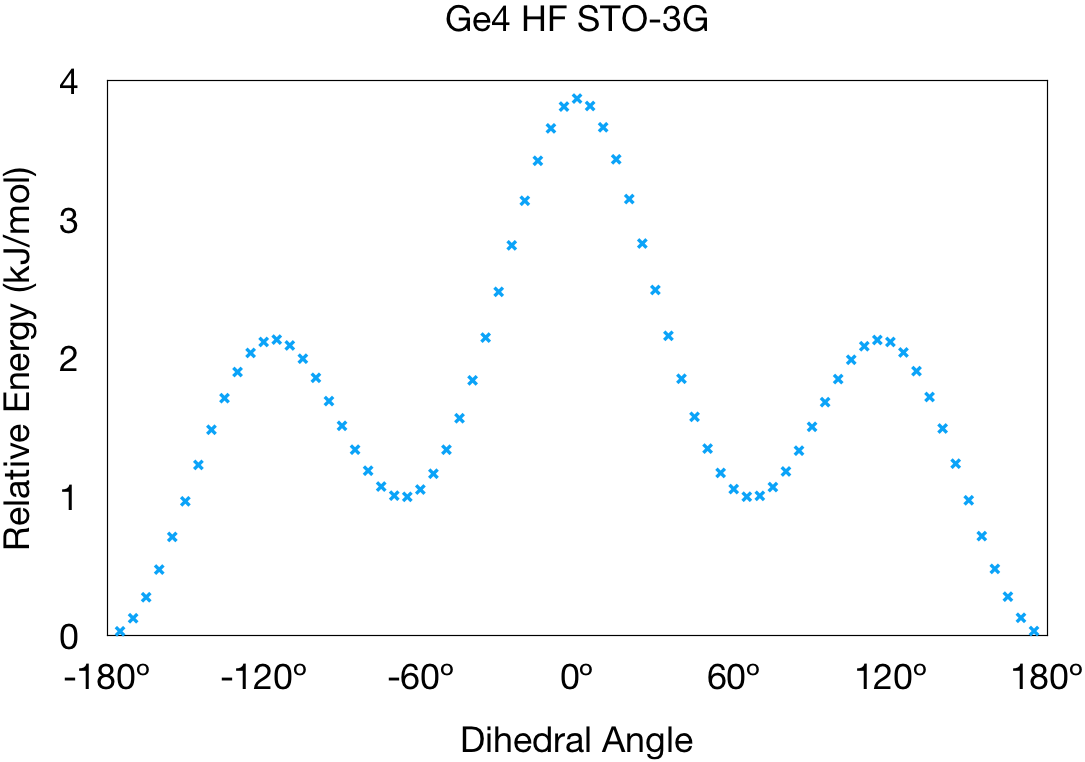
\includegraphics[width=0.75\textwidth]{Ge4HFSTO3G.png}
	
	\caption{Sample torsion plot at reduced energy scale.}
	
	\label{fig:EXTorsion}
	
\end{figure}

For a full comparative set, 3456 points of analyzed data were generated for each reference molecule's free energy in comparison with the others. 
Unsurprisingly, no simple correction factor arose by method of a simple additive or multiplicative term applied toward all torsion points. 
To expand on the comparative set, a set of butyl- group IV conformers were generated with every possible permutation of C, Si, and Ge, each then rotated about the torsion in 5$^{\circ}$ increments to produce a total 5832 conformers.
These were then subject to the same data comparison method as before, again to no noticeable trend.
A future avenue of research could be to further explore this with depressive or polynomial terms to discover whether a simple corrective function might exist with specific molecules.

While this approach likewise did not find any simple correction factor, a graphical representation of multiple functionals across the butyl C, Si, and Ge show an interesting trend, as visualized by a graph provided by Dr. Christopher Fennell and shown in figure \ref{fig:FennellTorsion}.
\begin{figure}
	
	\centering
	
	\makebox[\textwidth][c]{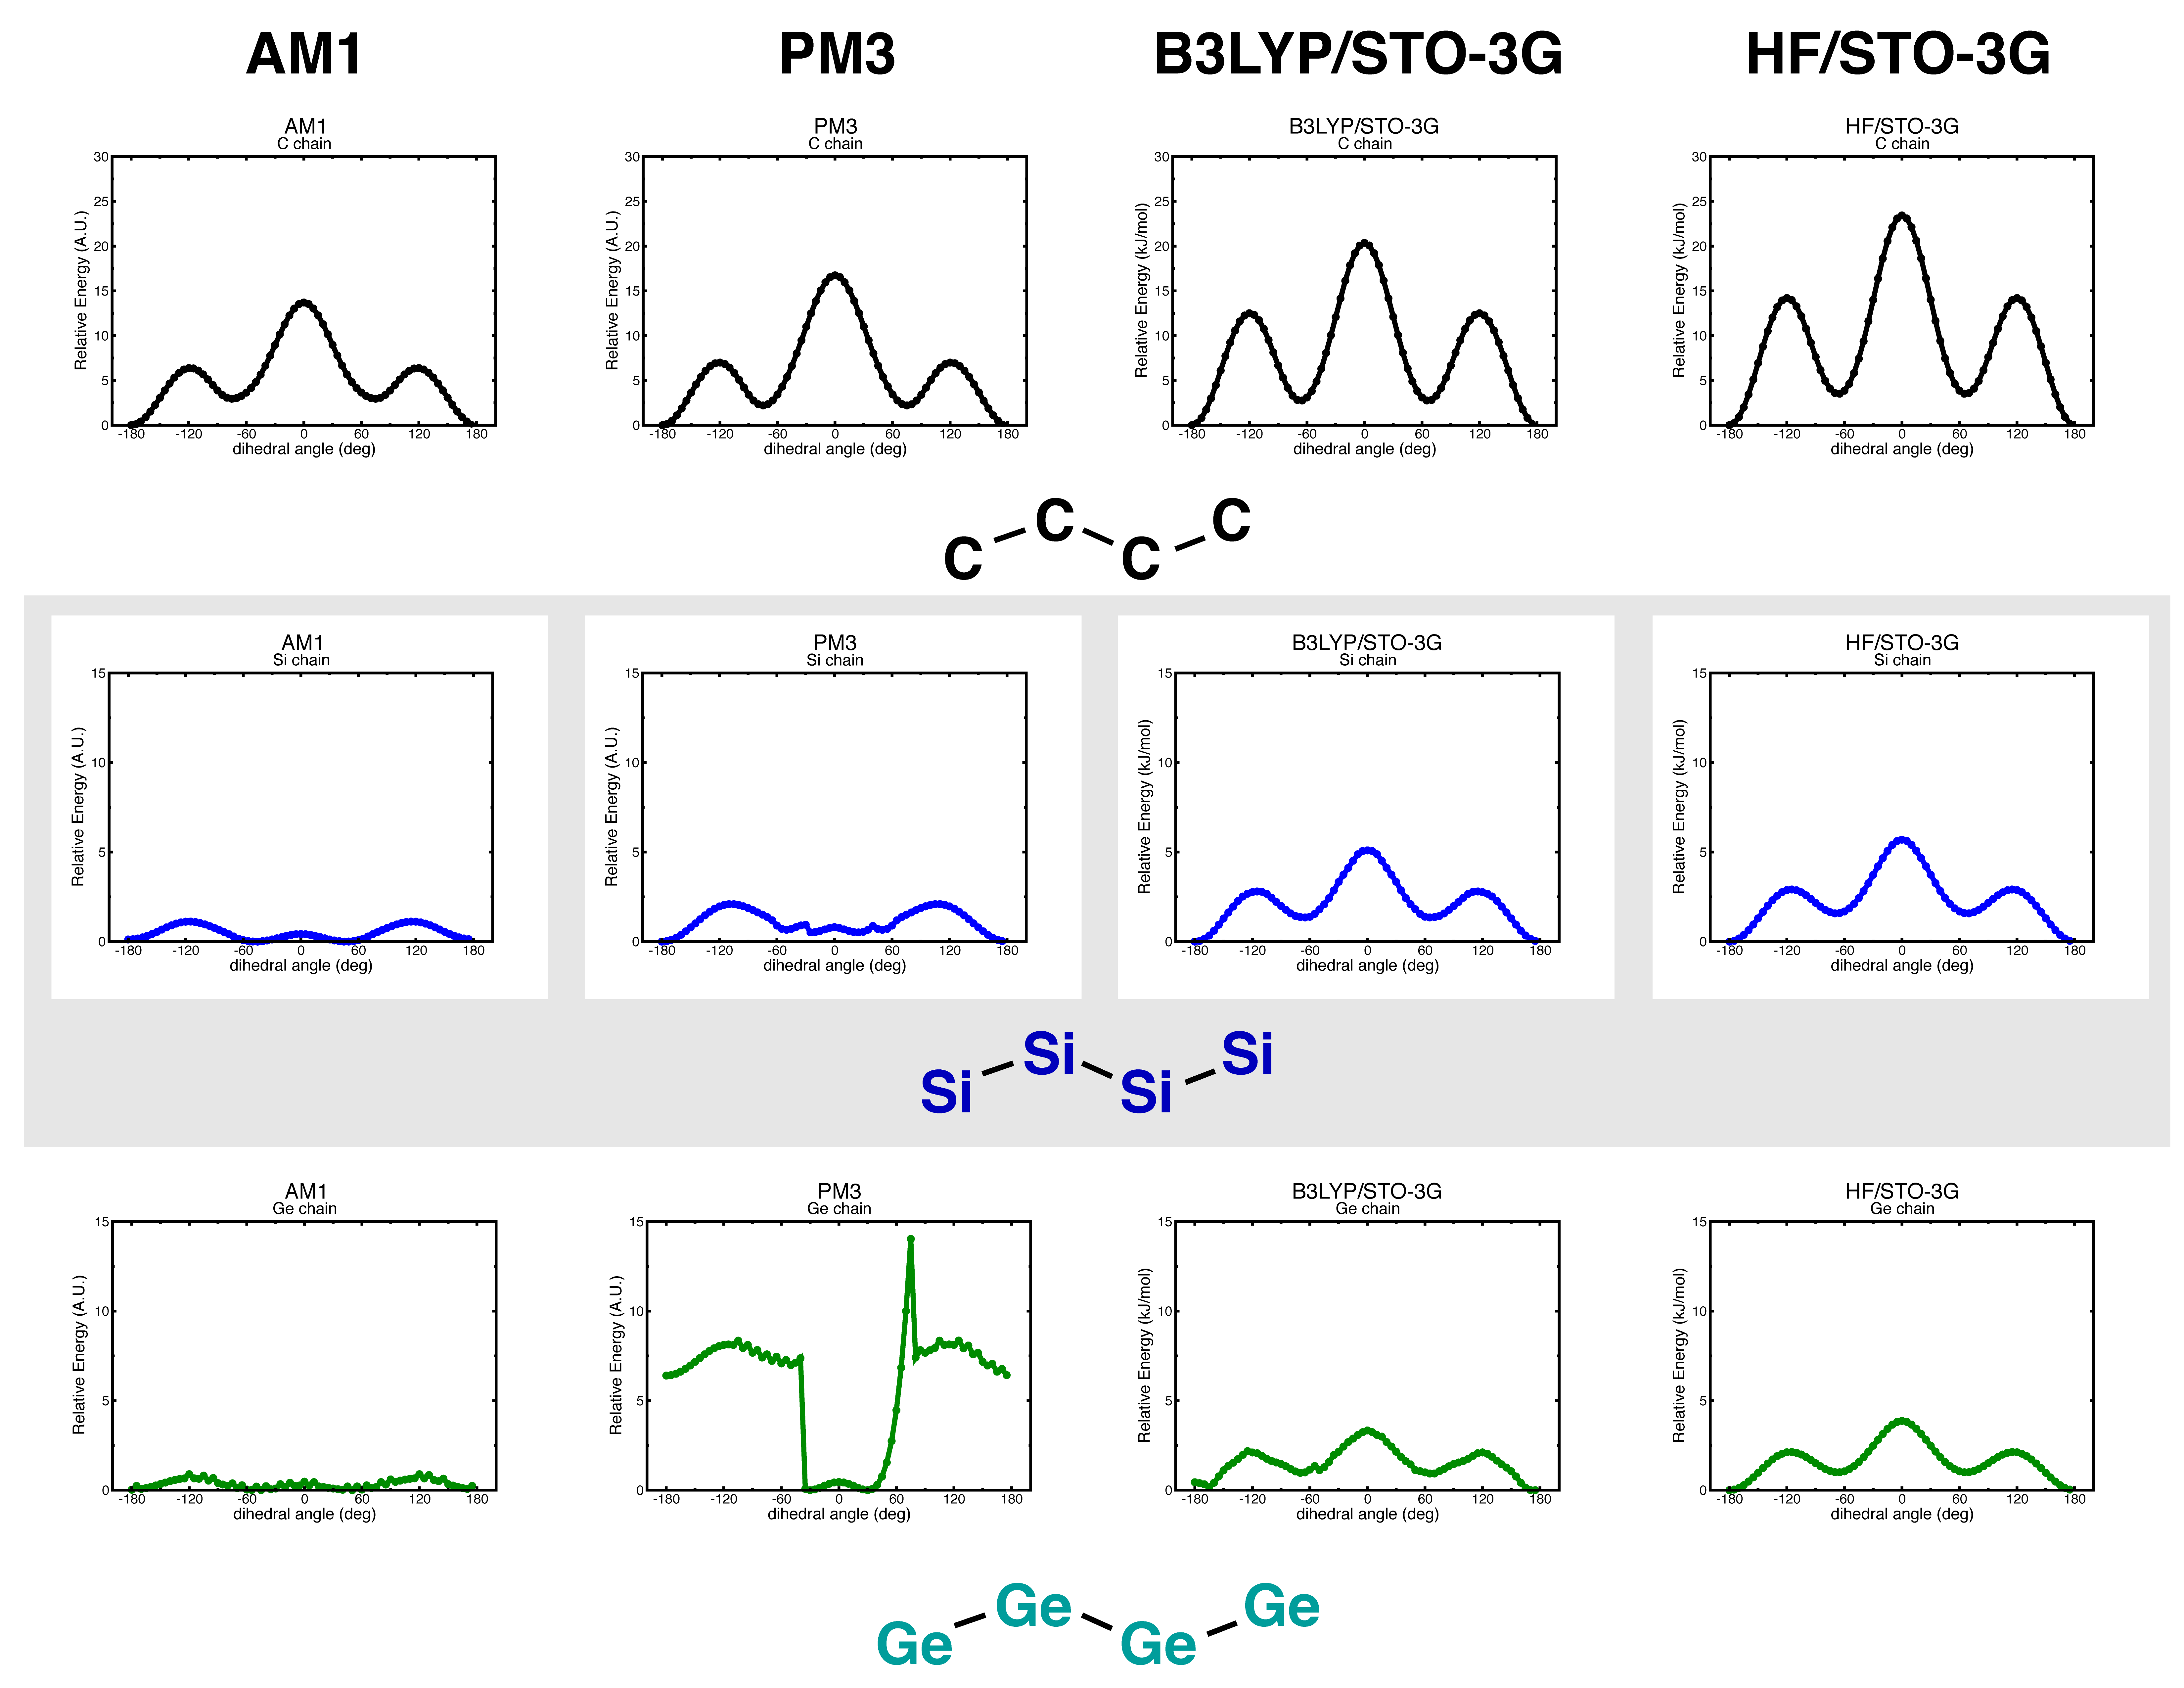
\includegraphics[width=1.3\textwidth]{FennellTorsion.png}}
	
	\caption{Visualization of a multiple pure group IV torsions at various theories and basis sets}
	
	\label{fig:FennellTorsion}
	
\end{figure}
A common theme of these graphs is that the relative energies follow the expected energetic barrier of a Newman projection, with local maxima at the 120$^{\circ}$ and 240$^{\circ}$ (or -120$^{\circ}$) angles and local minima at the 60$^{\circ}$ and 300$^{\circ}$ (or -60$^{\circ}$).
The global maximum and minimum were consistently at 0$^{\circ}$ and 180$^{\circ}$ angles, respectively.
As expected by different types of calculations, the torsion graphs hold different internal relative energies. 
For carbon, all four functionals produced a clean curve. 
The AM1 and PM3 functionals produced unexpected results for both Si and Ge graphs. 
In each, the expected highest energy 0$^{\circ}$ torsion angle was instead the most favorable of the three eclipsed angles.
Additionally, the Si PM3 and the Ge AM1 and PM3 functionals showed strong spikes along the expectedly smooth curve, with the Ge PM3 being noticeably broken.

While the Si graphs smoothed out for the B3LYP and HF functionals at STO-3G basis set, the Ge B3LYP showed significant spikes and only the HF STO-3G exhibited a smooth curve.
Effectively, this discovery of spikes along torsion drives led to the realization that the validity of a basis set could possibly be determined by the smoothness of a torsion drive.
For example, any calculation of a germanium-containing molecule will likely not produce reliable results with a B3LYP hybrid functional and STO-3G basis set, while the Hartree Fock STO-3G calculation would at least be tentatively reliable for comparative energy levels at various conformations.


\section{Discovery of a Consistent Inconsistency}

The next natural step was to calculate and plot additional functional theories and basis sets with the butagermanium chain. 
While effectively a lightly guided meandering through the available calculation types, the first effort was to observe relative differences across multiple basis sets of the Hartree Fock theory and to examine the relative computational requirements of each.
This plan was quickly redirected, however, when a curiosity within the data was revealed.

While running additional torsion drives of butagermane at differing basis sets and functional theories, an inverted energy was discovered. 
As can be seen in figure \ref{fig:geTorsFirst}, the B3LYP theory with 6-31G(d) basis set appears flipped upon a cursory glance. 
After a more careful observation, the minima and maxima are at the "wrong" angles and cannot be a simple flip of the minima and maxima.
Instead, the data is simply junk.

\begin{figure}
	
	\centering
	
	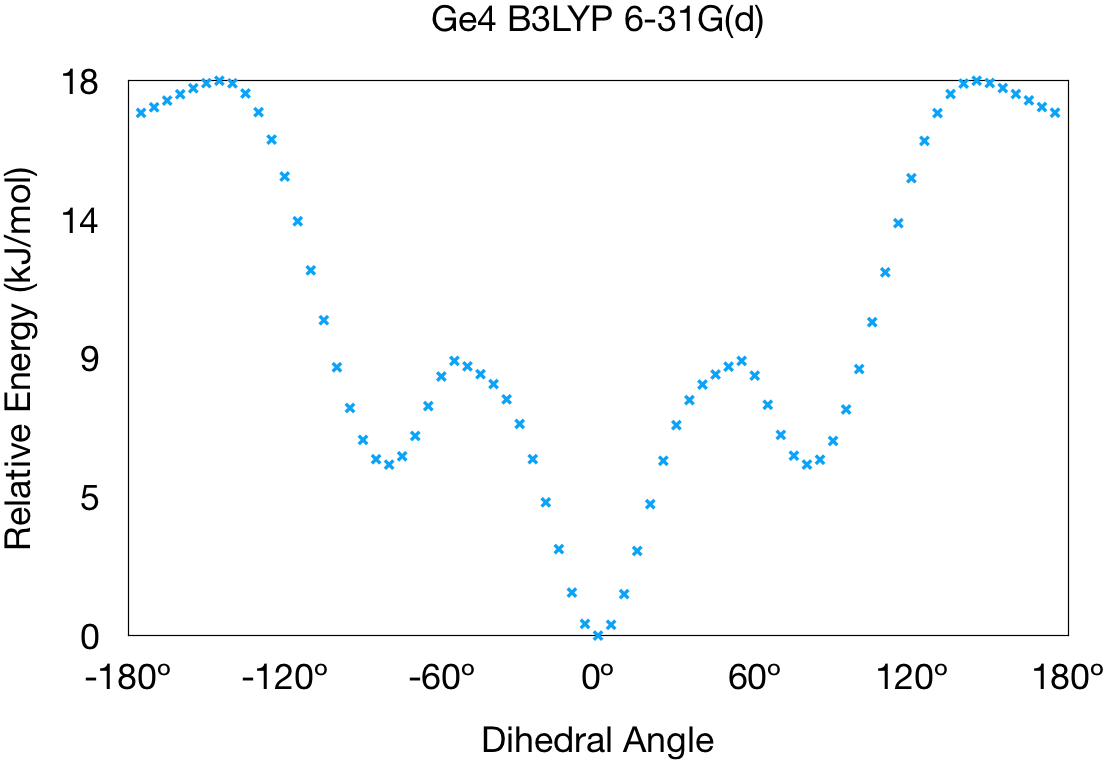
\includegraphics[width=0.75\textwidth]{geTorsFirst.png}
	
	\caption{A curious seemingly-inverted torsion plot of butagermane.}
	
	\label{fig:geTorsFirst}
	
\end{figure}

Naturally, the focus shifted toward discovering the source of the bad data.
A repeat of the trial yielded the same data.
A repeat of the system with a freshly created butagermane yielded the same data.
A trial with data from a butagermane trial with the 6-31G(d,p) basis set yielded the same data.
Each attempt at a 6-31G(d) basis set with the B3LYP theory yielded junk data, while other basis sets within the theory produced expected data. 
Next, the butagermane torsions were run with an identical basis set group with the Hartree-Fock theory, the results of which are shown in table \ref{fig:geTorsOne}.

Surprisingly, the 6-31G(d) result was also strangely inverted.
This process was repeated for several more theories, with the 6-31G(d) basis set results plotted in figure \ref{fig:geTorsAll}.
Curious to see if the germanium atom's basis set data or if the entire basis set method was the source, a similar run with butasilane was made and graphed in figure \ref{fig:siTorsOne}, to expected results.
A quick run confirmed the problem to also exist on Gaussian 03 as well as Gaussian 09.
The final effort was to check whether this error was isolated to Gaussian 09 or to all QM programs. 
A simplified test to calculate the energy of the expected global minimum (180$^{\circ}$) and maximum (0$^{\circ}$) of a Hartree Fock theory with the suspect 6-31G(d) basis set was prepared and executed, with the results tabulated in \ref{tab:geHFAppData}.
As can be seen, critical energetic difference was negative for Gaussian 09 and positive for both GAMESS and NWChem.
Since the expected conformations should yield a positive difference, it was concluded that both Gaussian 03 and 09 contain bad 6-31G(d) basis set data for germanium.

\begin{figure}
	
	\centering
	
	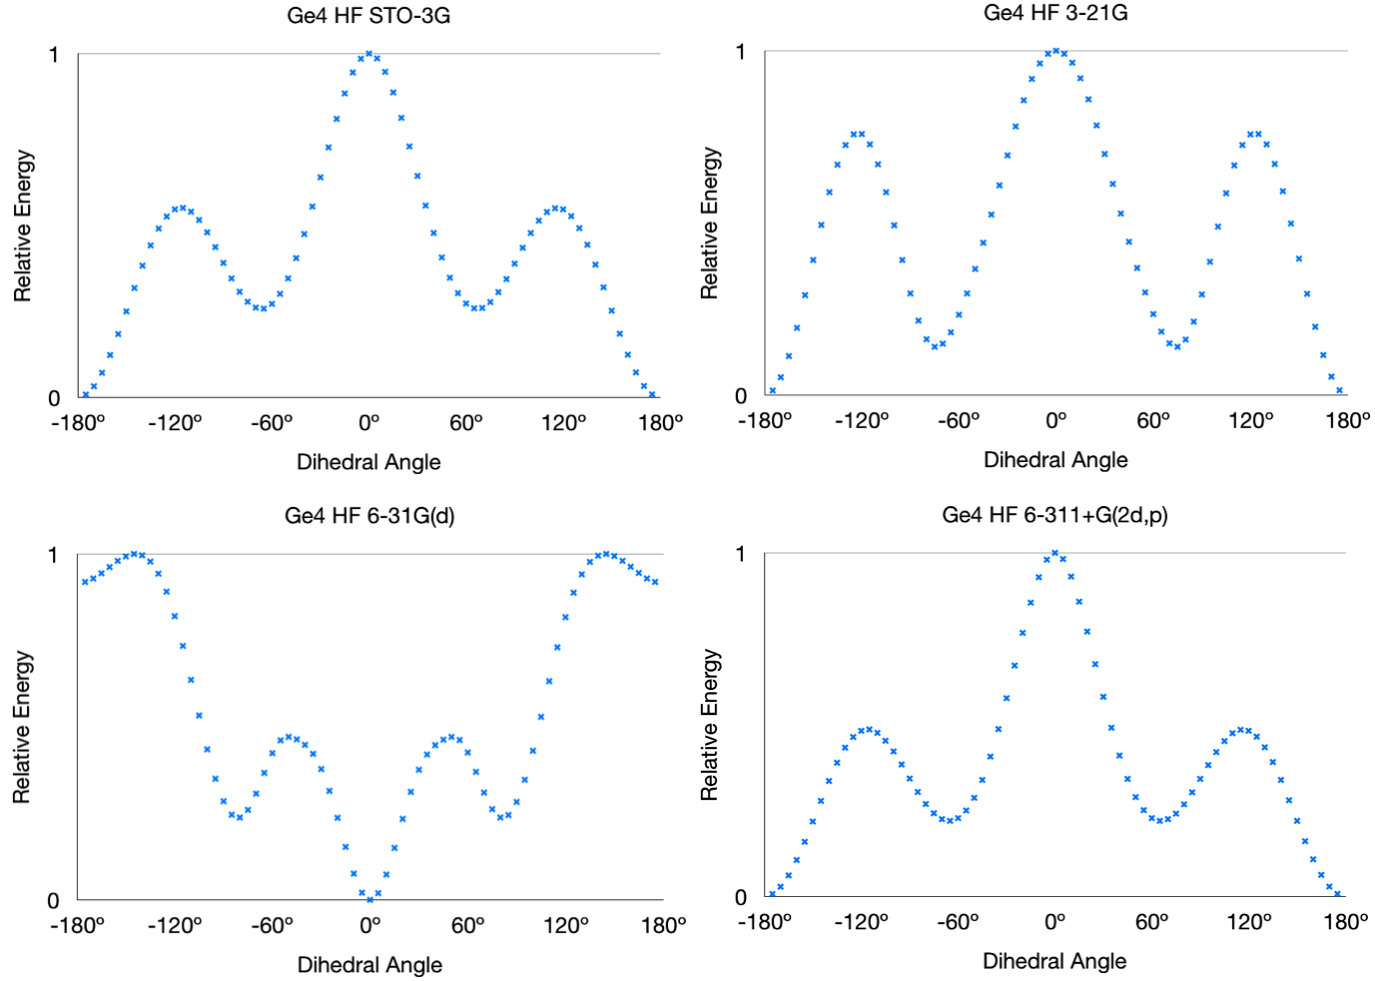
\includegraphics[width=\textwidth]{geTorsOne.png}
	
	\caption{Hartree Fock energy minimization of butagermane torsion run at varying basis sets.}
	
	\label{fig:geTorsOne}
	
\end{figure}

\begin{figure}
	
	\centering
	
	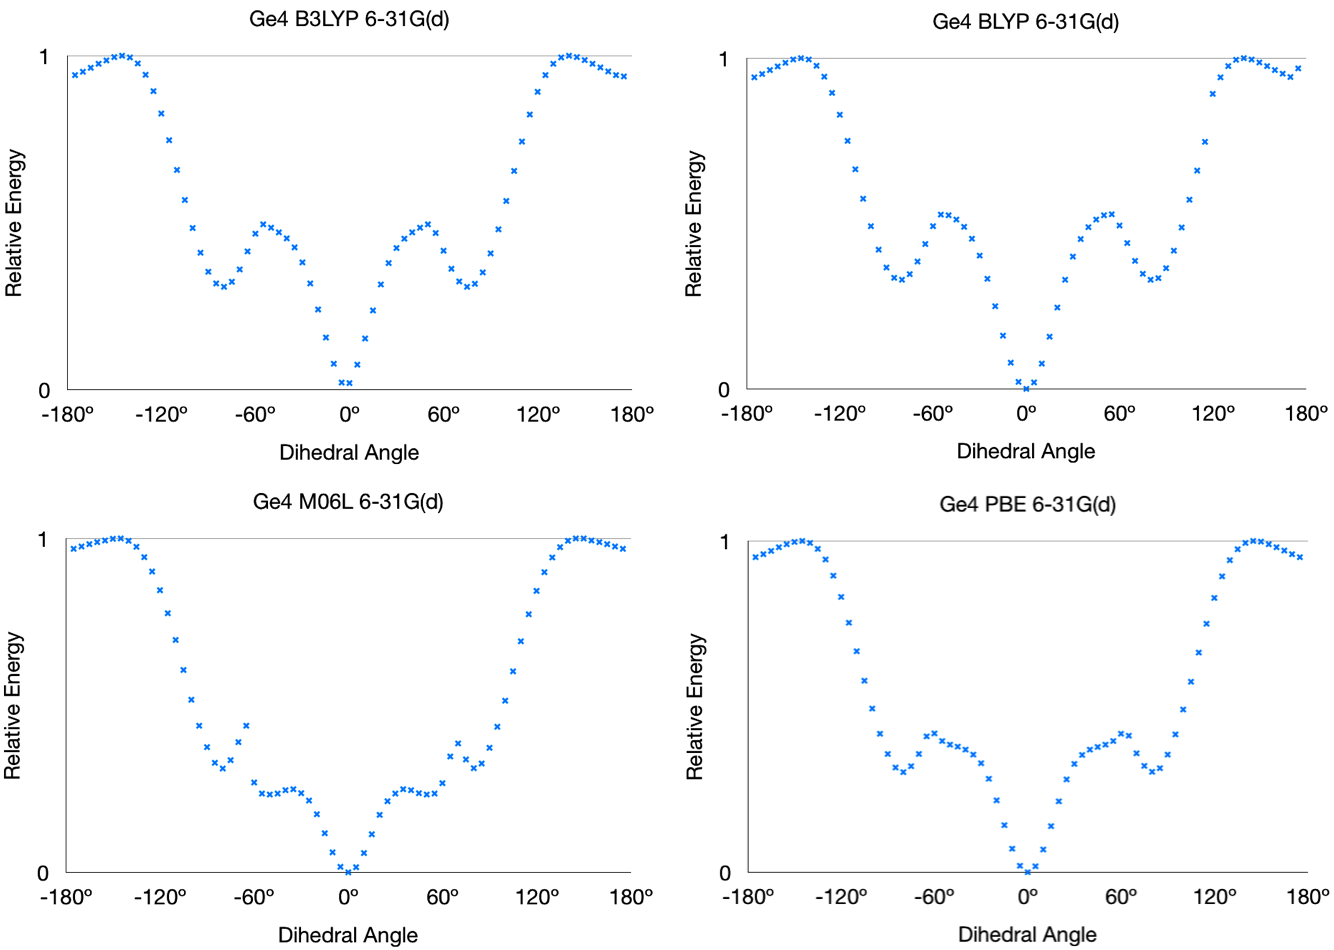
\includegraphics[width=\textwidth]{geTorsAll.png}
	
	\caption{Minimization of butagermane torsion run at varying theories and the 6-31G(d) basis set.}
	
	\label{fig:geTorsAll}
	
\end{figure}

\begin{figure}
	
	\centering
	
	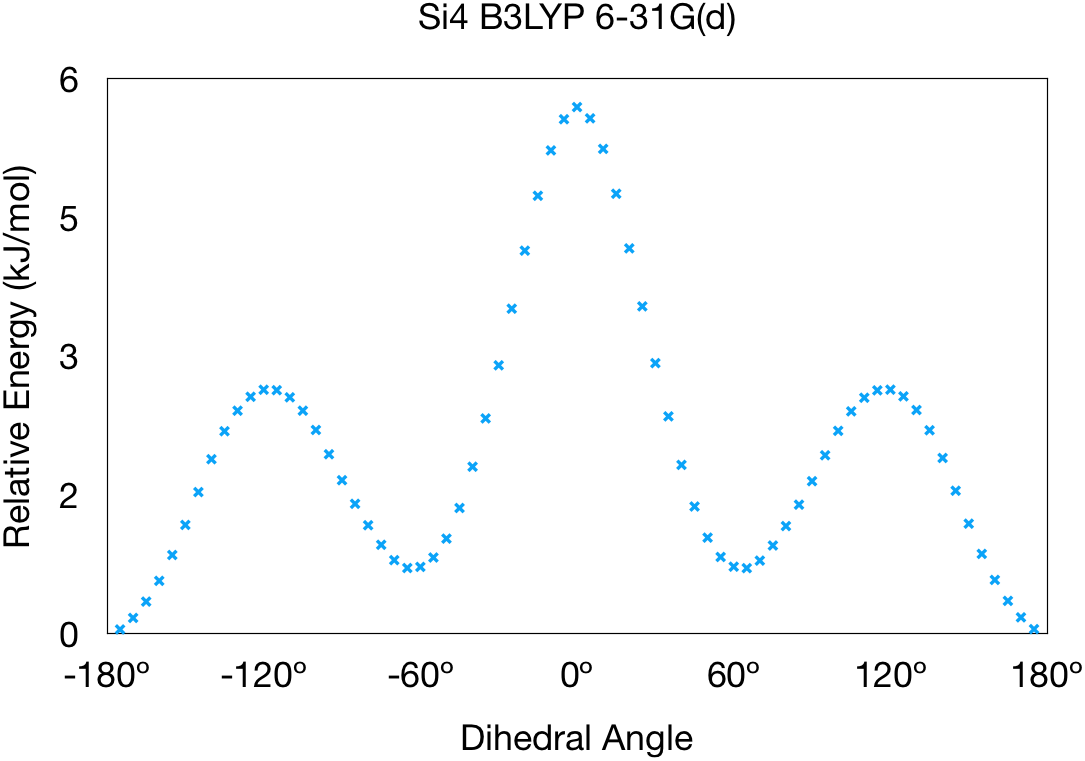
\includegraphics[width=0.75\textwidth]{siTorsOne.png}
	
	\caption{B3LYP energy minimization of butasilane torsion run at 6-31G(d) basis set.}
	
	\label{fig:siTorsOne}
	
\end{figure}


\begin{table}[]
	\centering
	\begin{tabular}{lllll}
		Program & \begin{tabular}[c]{@{}l@{}}Trans Energy\\ (Hartree)\end{tabular} & \begin{tabular}[c]{@{}l@{}}Cis Energy\\ (Hartree)\end{tabular} & \begin{tabular}[c]{@{}l@{}}∂ Energy\\ trans - cis\\ (Hartree)\end{tabular} & \begin{tabular}[c]{@{}l@{}}∂ Energy\\ trans - cis\\ (kcal / mol)\end{tabular} \\ \hline
		\multicolumn{1}{l|}{Gaussian} & -8298.8259 & -8298.8268 & -0.0009 & -0.5775 \\
		\multicolumn{1}{l|}{GAMESS} & -8306.1290 & -8306.1290 & 0.0040 & 2.4975 \\
		\multicolumn{1}{l|}{NWChem} & -8306.1290 & -8306.1250 & 0.0040 & 2.4974
	\end{tabular}
	\caption{Energy comparison of HF theory with 6-31G(d) basis set across multiple computational programs. The expected ∂E should be positive.}
	\label{tab:geHFAppData}
\end{table}

\section{Final Thoughts}

Unfortunately, a trend for simplifying the computation requirements of germanium was not discovered.
While it may exist among the data as a more involved function or as some other representation, there also may very well be no simple trend for switching between germanium and another group IV element.

On a much more interesting note, the results of the torsion drives revealed that Gaussian 03 and 09 contain some mistake within the 6-31G(d) basis set data for germanium. 
Considering the popularity of Gaussian software in computational chemistry, there are concerning implications about reliability of data for any germanium energy data with the 6-31G(d) basis set. 
Given that the torsion tests produced expected data for 6-31G(d) data subsequently run through a higher or lower basis set, only reported data with 6-31G(d) as the final calculated energy need be considered.
It is recommended that any investigator into computational aspects of germanium either replace the basis set data, use another basis set, or instead use a program like GAMESS or NWChem for that final computation.



